\section{MP visibility in the Llama Base-to-Instruct checkpoint delta}
\label{sec:spectral}

We begin with the broadest empirical question: does a real post-training update
contain components that are visible under the fitted reference? We analyze the
increment $\dW$ for all seven linear maps in each of the $32$ decoder layers of
Llama-3-8B \citep{grattafiori2024llama3}, $224$ matrices in total. For each
matrix, we compare the eigenvalues of
$C = \tfrac1p \dW^{\!\top}\dW$ with a Marchenko--Pastur visibility reference fit
to its bulk (Section~\ref{sec:theory}; Appendix~\ref{app:details}). The
content-addressed analysis manifest in the appendix indexes the committed sweep,
summaries, and producing code.

\paragraph{Every analyzed Llama increment matrix has an MP-visible leading eigenvalue.}
The leading eigenvalue of $C$ exceeds the operational Marchenko--Pastur
visibility threshold in all
$224$ matrices. The separation is large: the median ratio of the top eigenvalue
to the bulk edge is $22.0$, it exceeds $5$ in $216/224$ matrices, and its tail
reaches $2.45\times 10^4$. Under the fitted Gaussian/MP visibility reference, a
structureless increment would place the top eigenvalue near the edge, at ratio
$1$, compared with the observed median of $22.0$. Figure~\ref{fig:spectrum}
shows a representative near-zero Marchenko--Pastur bulk with several separated
leading eigenvalues. An iid Gaussian matrix whose entry variance is set to the
median-matched MP bulk estimate reproduces the fitted bulk but has no
MP-visible leading values (Figure~\ref{fig:nullcompare}). The Gaussian control
illustrates departure from an iid diffuse reference; matched real fine-tunes test
whether the pattern generalizes.
As a fit-sensitivity check, an all-spectrum trace-moment scale, deliberately
inflated by the spikes, still places every leading eigenvalue above its fitted
edge and gives a median top-to-edge ratio of $11.8$. This top-edge ratio is an
algebraic function of stable rank and is not independent robustness evidence.
The full-spectrum exceedance counts do add a separate fit-sensitivity check and
change substantially (Appendix~\ref{app:details}).
Across both fits, the stable conclusion is qualitative: the real checkpoint
delta contains directions too prominent to treat as diffuse noise. This makes
them candidates for behavioral tests, not evidence that they encode alignment.

\begin{figure}[t]
\centering
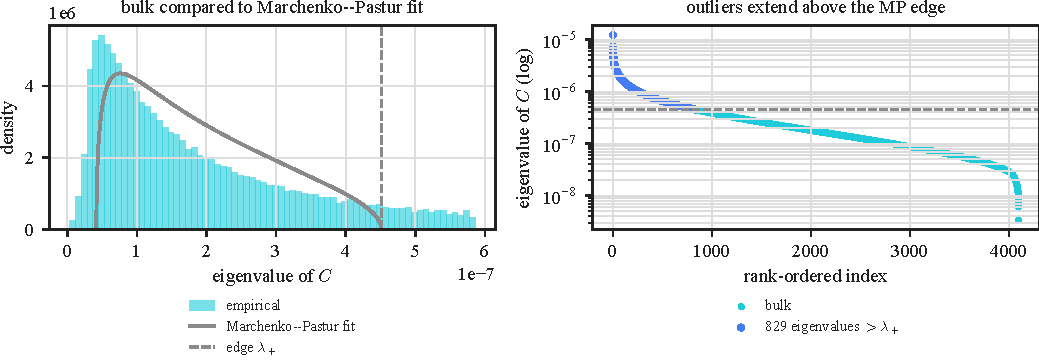
\includegraphics[width=0.92\textwidth]{../results/figures/bulk_spikes.pdf}
\caption{Spectrum of the Base-to-Instruct checkpoint delta for a representative matrix
(\texttt{gate\_proj}, layer 15; all $4096$ eigenvalues of $C$). \emph{Left:} the
eigenvalue-density bulk has a heavier right tail than the Marchenko--Pastur fit.
\emph{Right:} eigenvalues run largest to smallest; higher is stronger. Points
above the horizontal line exceed the raw fitted MP edge. Of $4096$
eigenvalues, $829$ exceed $\lambda_+$ and $821$ exceed the operational
edge-plus-six-fluctuation-scale threshold; the largest is $27\times$ the
edge. The refusal and misalignment interventions below test the behavioral
relevance of these spectral components.}
\label{fig:spectrum}
\end{figure}

\begin{figure}[t]
\centering
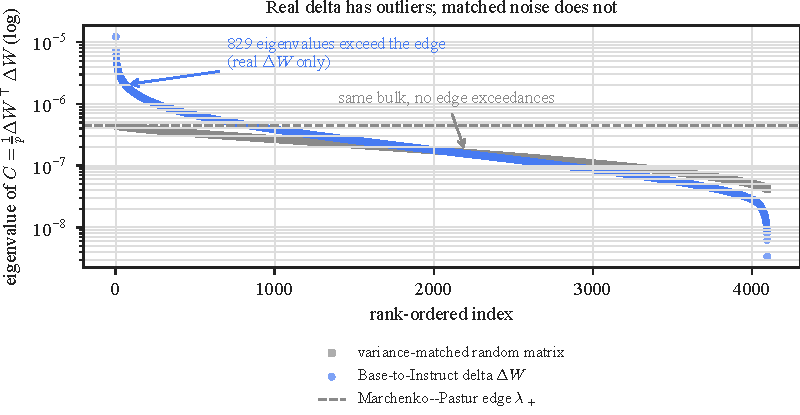
\includegraphics[width=0.62\textwidth]{../results/figures/spectrum_null.pdf}
\caption{Ranked eigenvalues for the same increment (circle markers) and a
Gaussian control at the fitted MP bulk scale (square markers): left is larger, higher is
stronger, and crossing the dashed edge marks visibility under the fitted
reference. Both share the bulk, but only the real increment exceeds the edge.
Matched fine-tunes provide the
empirical control beyond this Gaussian reference.}
\label{fig:nullcompare}
\end{figure}

The fitted Marchenko--Pastur curve answers visibility, not specificity. Learned
updates are non-exchangeable and neural-network spectra are already structured
\citep{martin2021}, including in transformers \citep{staats2024small}. We use
the Gaussian reference only as a diffuse null, then examine how the observed
structure is distributed before testing behavior.

\paragraph{The energy is concentrated.}
We call values above $\lambda_+$ raw MP-edge exceedances and values above
$\lambda_+$ plus six fitted finite-size scales operational visibility
exceedances. The median operational visibility-exceedance count is $709$, about
$19\%$ of matrix rank. This count depends on the fitted visibility threshold and
is not an estimate of algebraic signal rank.
The stable rank $\|\dW\|_F^2/\|\dW\|_2^2$ has median $109$. The $14336$
feed-forward width is a hidden dimension, while algebraic rank is bounded by
$\min(p,q)$: $1024$ for key/value projections and $4096$ for the other maps.
Matrix by matrix, median stable rank is $3.3\%$ of this ceiling, showing energy
concentration at every layer (Figures~\ref{fig:bylayer}
and~\ref{fig:spectral-landscape}). A small fraction of the available dimensions
therefore carries a disproportionate share of the update, making subspace-level
tests practical. Neither statistic identifies a mechanism, and both depend on
the chosen parameterization.

\paragraph{Query/key maps are most spectrally concentrated.}
Concentration varies across the seven maps
(Table~\ref{tab:bytype}). The query and key projections have the most extreme
top-to-edge ratios, with medians of $81$ and $25$, and the smallest stable
ranks ($45$ and $36$), making them the most concentrated of the seven map types.
The value and output-side maps spread their energy
more widely. Because query/key maps set attention patterns
\citep{vaswani2017attention}, they are natural places to look for structured
post-training change. The result does not show that attention-pattern changes
cause the behavior below, or reveal how many independent mechanisms produced
the update.

\begin{table}[t]
\centering
\caption{Spectral summary of the Base-to-Instruct checkpoint delta by matrix type.
Values are descriptive medians over the $32$ analyzed layers; query and key
projections are the most concentrated.}
\label{tab:bytype}
\small
\begin{tabular}{lccc}
\toprule
matrix & median top/edge & median operational exceedances & median stable rank \\
\midrule
\texttt{q\_proj}    & $80.9$ & $808$ & $45.0$ \\
\texttt{k\_proj}    & $25.4$ & $238$ & $36.1$ \\
\texttt{v\_proj}    & $6.2$  & $168$ & $99.9$ \\
\texttt{o\_proj}    & $23.6$ & $756$ & $115.0$ \\
\texttt{gate\_proj} & $24.6$ & $734$ & $111.6$ \\
\texttt{up\_proj}   & $18.4$ & $778$ & $147.9$ \\
\texttt{down\_proj} & $8.1$  & $680$ & $298.9$ \\
\bottomrule
\end{tabular}
\end{table}

\begin{figure}[t]
\centering
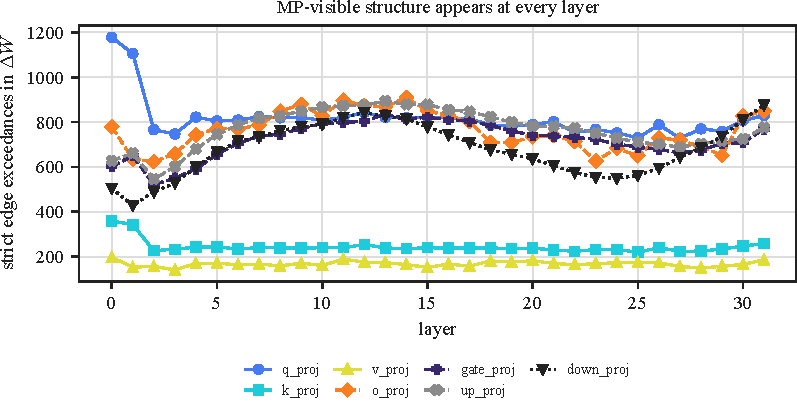
\includegraphics[width=0.78\textwidth]{../results/figures/spikes_by_layer.pdf}
\caption{Operational visibility-exceedance counts in $\dW$ by layer and matrix
type. Rightward is deeper and higher means more directions above the fitted edge
plus six finite-size scales. Every layer has visible structure. These counts
depend on the fitted visibility threshold and need not equal signal rank. The
layer-wide recurrence rules out an isolated single-layer phenomenon under this
reference, but not generic fine-tuning structure.}
\label{fig:bylayer}
\end{figure}

\begin{figure}[t]
\centering
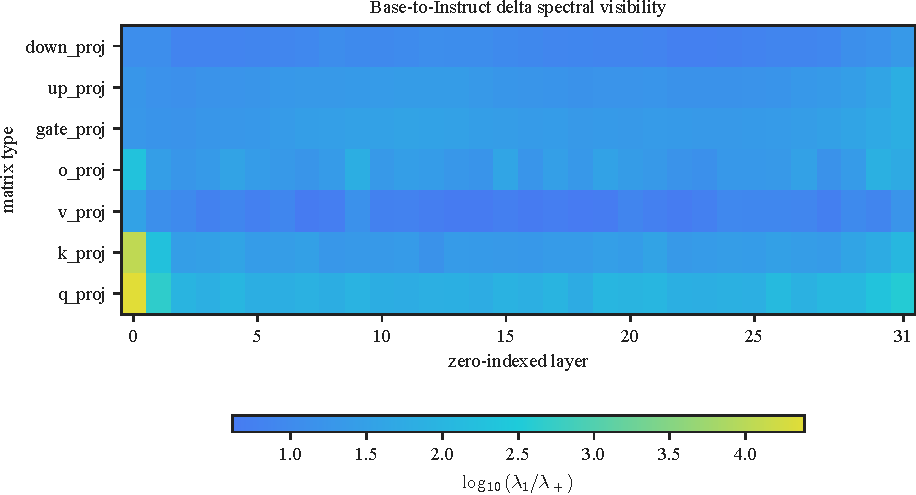
\includegraphics[width=0.74\textwidth]{../results/figures/spectral_landscape.pdf}
\caption{Heatmap of $\log_{10}(\lambda_1/\lambda_+)$ across all $224$
increments. Columns are zero-indexed layers and rows are matrix types; lighter
colors indicate greater separation above the fitted MP edge. This summarizes
spectral visibility, not behavioral relevance.}
\label{fig:spectral-landscape}
\end{figure}

\paragraph{The delta has little overlap with the base model's dominant subspace.}
To distinguish new directions from rescaling of existing ones, we compare for
each attention-output map the
top-$16$ left-singular subspace of the increment with the top-$16$ left-singular
subspace of the base weight, by mean squared principal-angle cosine
(Figure~\ref{fig:energy}, right). For orthonormal bases $U,V\in\R^{d\times16}$,
the statistic is $\|U^\top V\|_F^2/16$; its independent-random expectation is
$16/d=0.0039$ at $d=4096$. The observed median is $0.0134$ across layers,
versus $0.00395$ for the seeded random controls, a $3.39\times$ ratio and far below the value a
rescaling of dominant base directions would produce. The delta therefore has
little alignment with the base weight's dominant singular directions, with the
largest departures at the first layers and the final layer. The left panel of
Figure~\ref{fig:energy} shows how front-loaded the increment energy is:
for the query projection the top $64$ of $4096$ singular directions already carry
a third of $\|\dW\|_F^2$. Operationally, the useful candidates come from the
update itself; simply inspecting the base model's dominant modes would miss
most of the observed change.

\begin{figure}[t]
\centering
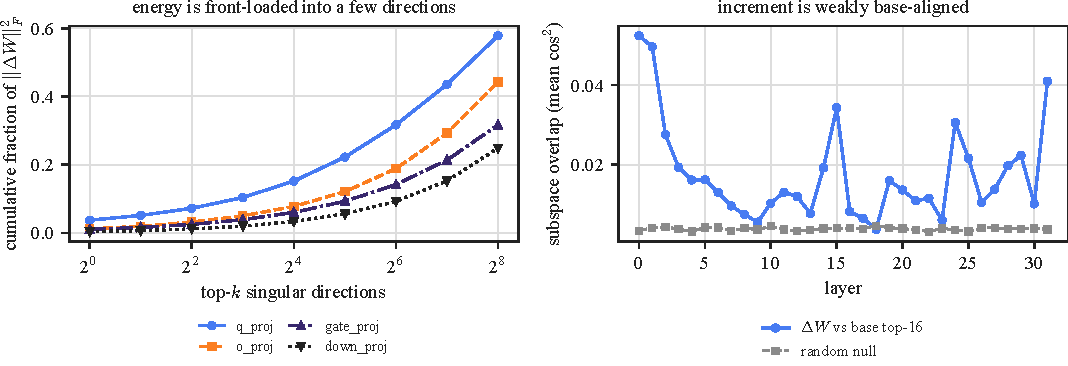
\includegraphics[width=0.96\textwidth]{../results/figures/energy_overlap.pdf}
\caption{\emph{Left:} cumulative increment energy averaged over the $32$
layers within each matrix type; rightward includes more singular directions
and upward means more energy captured. \emph{Right:} per-layer
top-$16$ increment--base overlap by layer: higher means stronger subspace
alignment. Energy is front-loaded, while overlap stays near the random null, so
the delta contributes concentrated directions not already dominant in the base
weight.}
\label{fig:energy}
\end{figure}

Because concentrated updates also arise from generic training variation
\citep{aghajanyan2021,hu2022lora}, we next test refusal and condition specificity.
